%------------------第三章---------------------------
\newpage
\section{超声波接近传感器硬件设计}

\subsection{超声波接近传感器控制电路设计}
本设计中所使用的CPLD芯片型号为EPM240T100C5N,涉及到的控制电路较简单,在最小系统板的基础上,增加了检测计数电路和TUSS4470外围电路。如图\ref{传感器整体原理图}为传感器整体的原理图\upcite{CPLD芯片设计指南}。
\begin{figure}[ht]
	\centering
	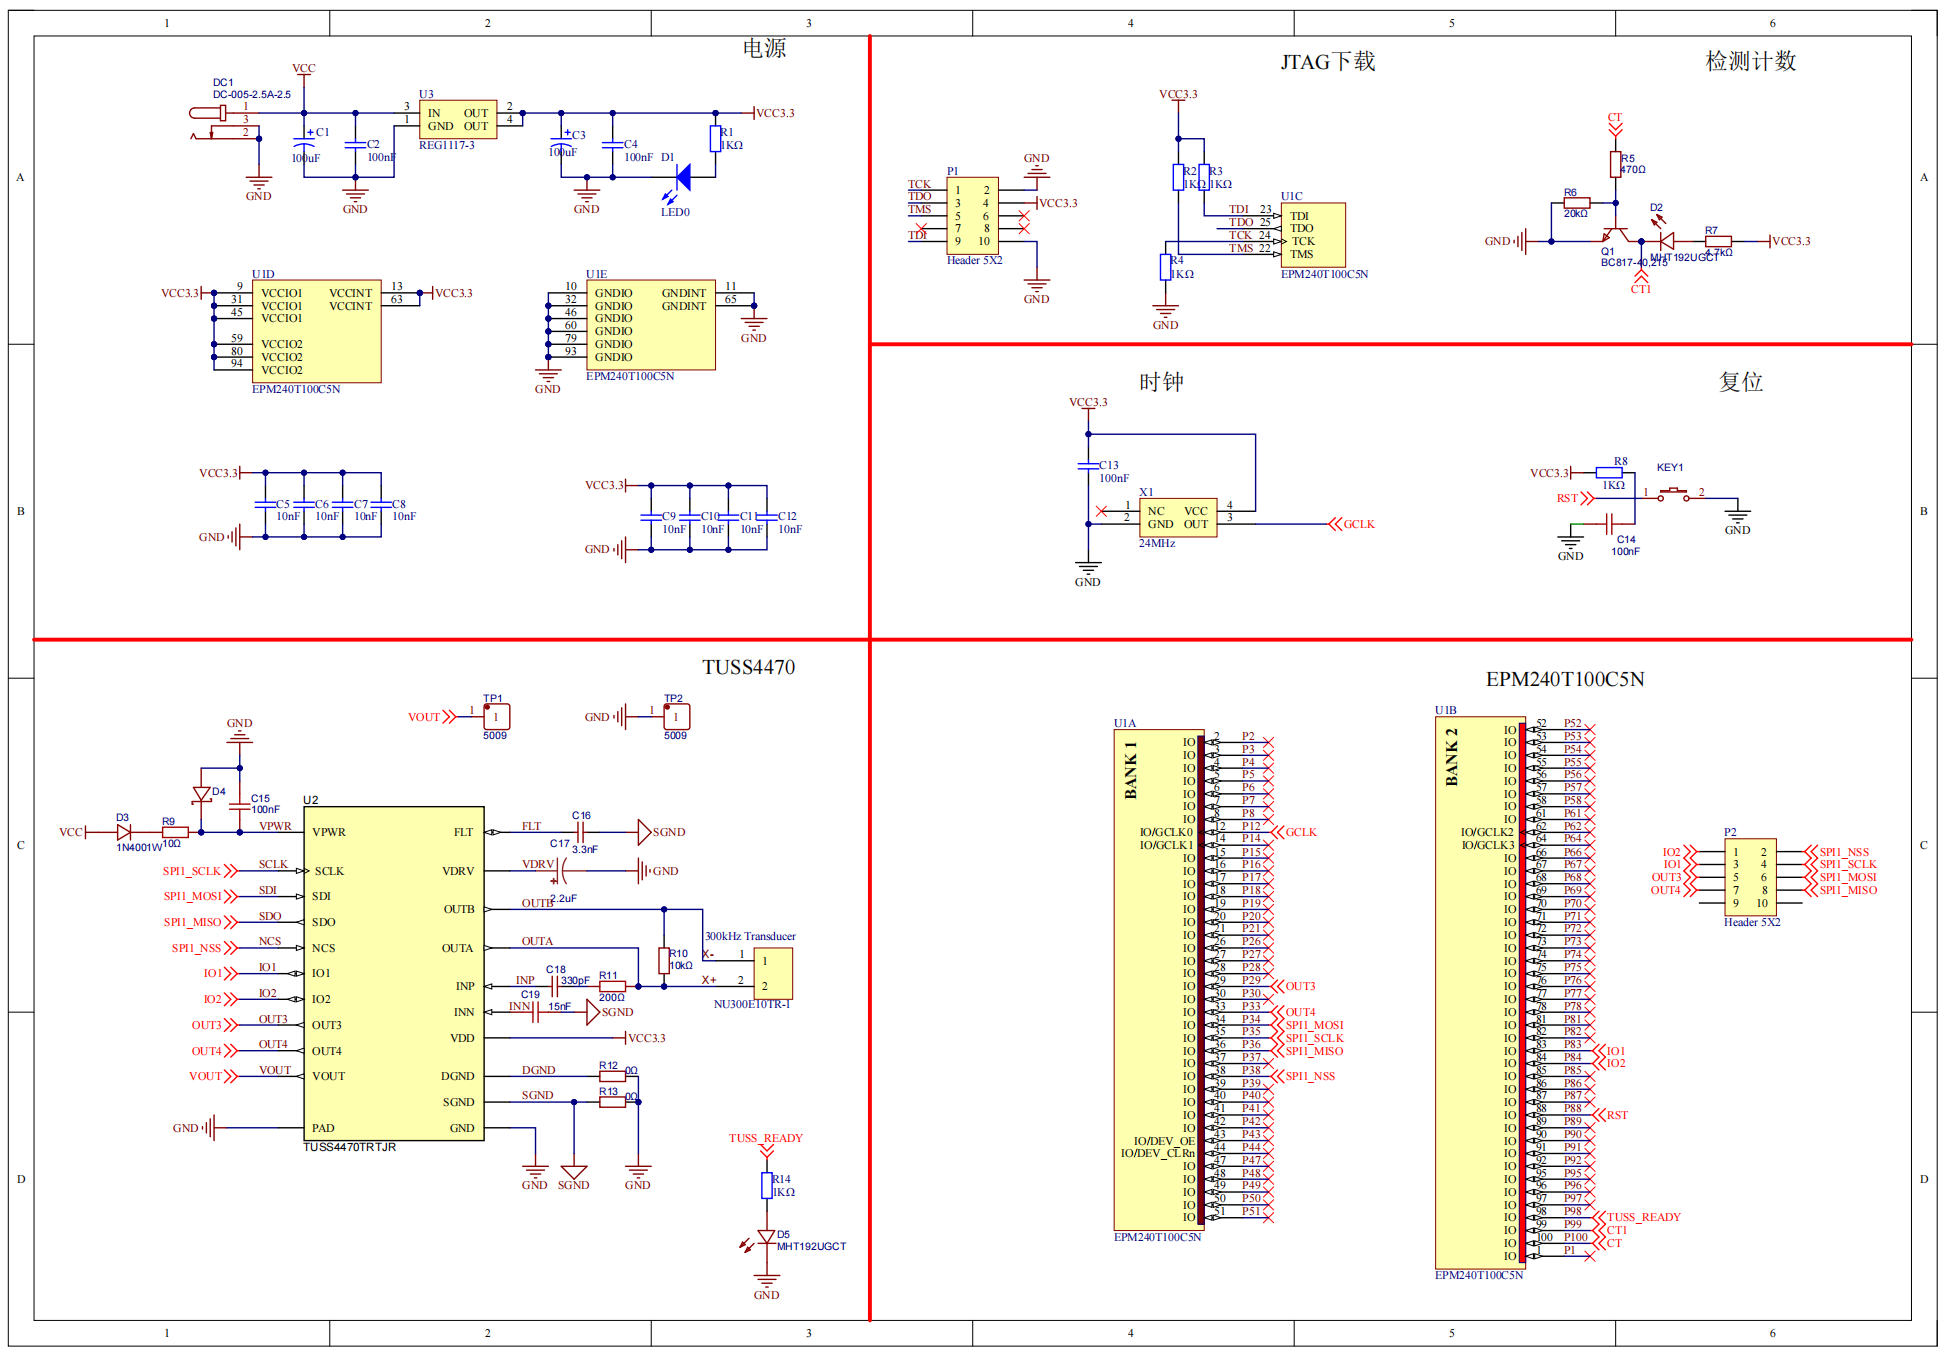
\includegraphics[width=12cm]{figure/Overall circuit.png}
	\caption{传感器整体原理图}
	\label{传感器整体原理图}
\end{figure}
\subsubsection{电源模块}
根据数据手册要求,可得知EPM240T100C5N的控制电压为3.3V
TUSS4470芯片的控制电压为3.3V,
超声探头的驱动电压为:5V-30V\upcite{超声探头手册}。
可得出电源的设计方案。电源由DC接口、降压芯片、滤波电容组成,可得到12V以及3.3V的电压为各模块供电。

\subsubsection{JTAG下载模块}
JTAG(Joint Test Action Group) 下载模块是一种用于编程和调试数字电路和嵌入式系统的通信接口,在本设计中JTAG主要用于烧录调试MCU代码。

\subsubsection{检测计数模块}
检测计数模块的功能在于,亮灯提示钢化玻璃到位,并对经过的玻璃进行计数。如图\ref{检测计数模块电路图},CT引脚为MCU输出信号,当程序确定检测到物体后,CT引脚电压拉高,LED灯亮,当物体离开检测范围后,LED灯灭。CT1引脚则是作为MCU的输入信号,当检测到一次物体后,CT1发出一次脉冲信号,计数加一,以此来实现计数功能。
\begin{figure}[ht]
	\centering
	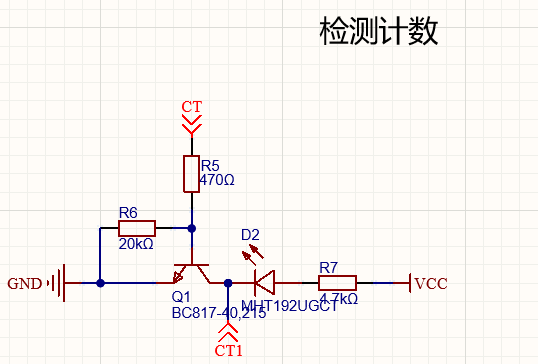
\includegraphics[width=7cm]{figure/detection count circuit.png}
	\caption{检测计数模块电路图}
	\label{检测计数模块电路图}
\end{figure}

\subsubsection{超声波接近传感器控制电路PCB设计}
在完成控制电路原理图的设计后,需要设计PCB部分。如图\ref{超声波接近传感器整体PCB设计}为传感器PCB整体设计图,图\ref{超声波接近传感器控制电路PCB设计}为控制电路PCB设计图。
\begin{figure}[ht]
	\centering
	\subfloat[超声波接近传感器整体PCB设计]{
		\begin{minipage}[b]{0.5\textwidth}
			\centering
			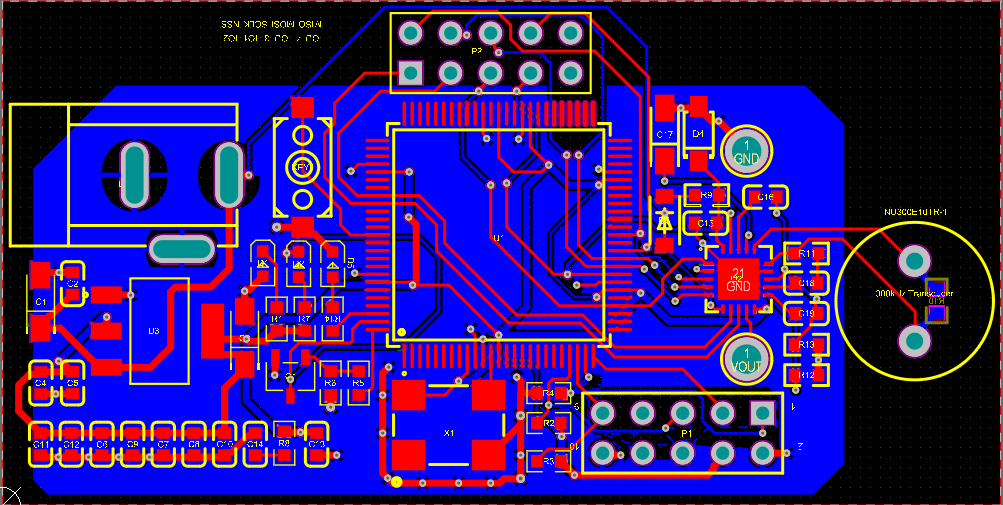
\includegraphics[height=4.5cm]{figure/overall pcb.png}
		\end{minipage}
		\label{超声波接近传感器整体PCB设计}
	}
	\subfloat[超声波接近传感器控制电路PCB设计]{
		\begin{minipage}[b]{0.5\textwidth}
			\centering
			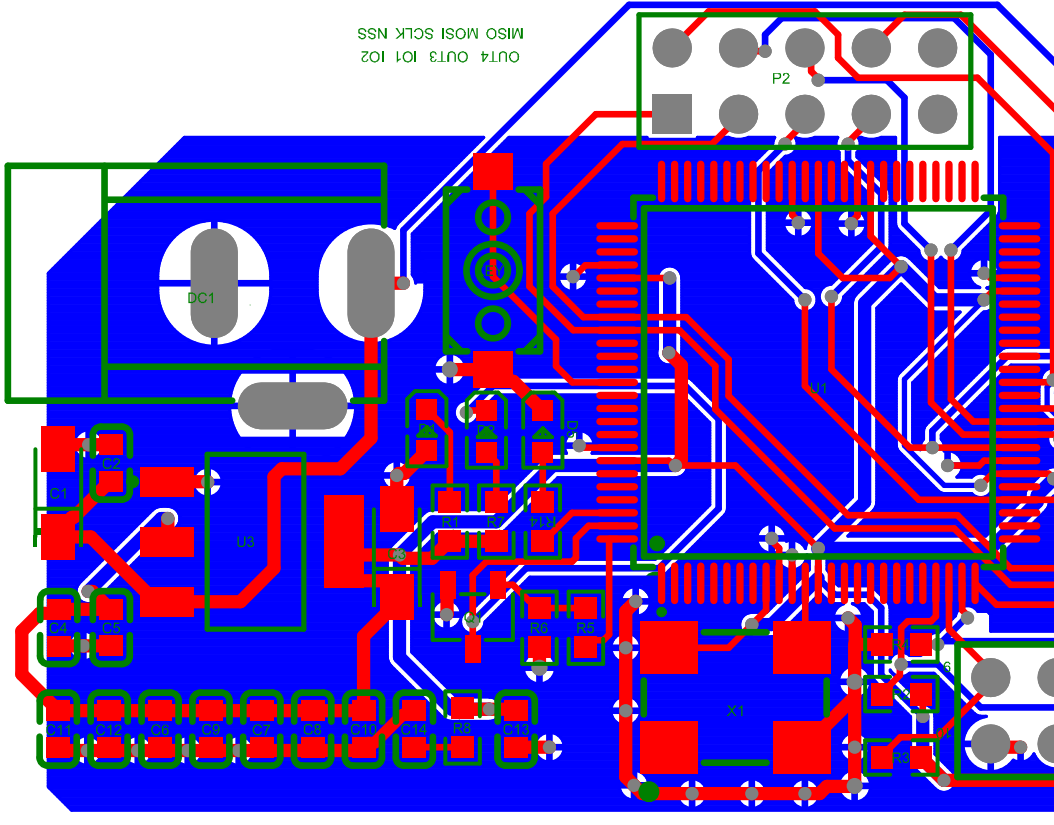
\includegraphics[height=4.5cm]{figure/cpld pcb.png}
		\end{minipage}
		\label{超声波接近传感器控制电路PCB设计}
	}
	\caption{超声波接近传感器PCB设计}
	\label{超声波接近传感器PCB设计}
\end{figure}
\paragraph{线宽}
对于功率较大的部分如电源、超声换能器驱动部分,需要对布线进行加宽处理,避免因发热而影响电路板正常工作,甚至产生损坏。\par
\paragraph{时钟包地处理}
对于速率较低的时钟,需进行包地处理,即在地线上等间距打过孔。包地的作用一是拉开与其他信号的距离,从而减小干扰;二作为自身参考和屏蔽。

\newpage
\subsection{TUSS4470芯片外围电路设计}


\begin{figure}[ht]
	\centering
	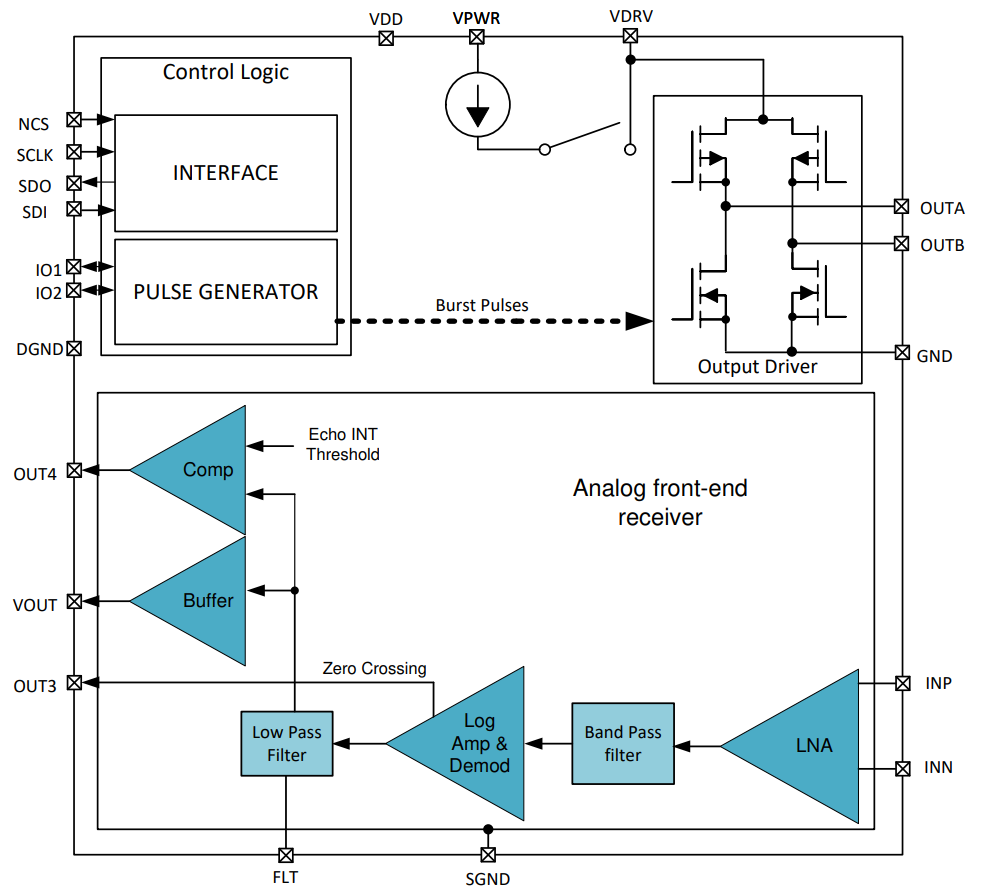
\includegraphics[width=12cm]{figure/Function Block Diagram.png}
	\caption{TUSS4470芯片功能框图\upcite{TUSS4470芯片手册}}
	\label{TUSS4470芯片功能框图}%文中引用该图片代号
\end{figure}
图\ref{TUSS4470芯片功能框图}为TUSS4470驱动芯片的整体功能框图\upcite{TUSS4470芯片手册},以此作为外围电路设计的参考资料。如图所示,芯片按照功能可分为逻辑控制、输出驱动、回波接收三个部分。其中逻辑控制部分又分为SPI通信和脉冲发生模块,SPI通信模块用于接收MCU芯片发送的芯片配置数据,脉冲发生模块的两个引脚IO1、IO2连接MCU芯片作为脉冲发生控制引脚,根据芯片不同的IO模式,两个引脚配合产生指定脉宽、脉冲数的脉冲信号;输出驱动模块的OUTA、OUTB引脚直接连接超声换能器,VDRV引脚连接外部电容,VPWR可对电容充电,在VDRV到达设定电压值后,VPWR停止对VDRV供电,这使得超声换能器的驱动电压可以保持在设定值,以此保证发出脉冲的声压水平可以稳定在一定水平,从而保证发射出稳定的脉冲波(其中VDRV的设定电压可通过SPI对芯片进行配置);回波接收模块的作用在于:对回波信号进行处理,输出可供MCU进行检测判断的信号其中INP、INN引脚连接超声波换能器的正负端,FLT连接外部电容作为低通滤波器对回波信号进行滤波处理。OUT3引脚内部连接至模块中的对数解调模块,当回波信号在模块内进完成放大进行解调时,将某阶段信号作为零点,输出过零信号,以验证接收信号的频率, 提高对其他信号的抗干扰性。OUT4作为检测到位的指示信号,当VOUT输出电压超过芯片配置数据中设定的阈值时,OUT4拉高。(VOUT引脚的电压值由公式\ref{VOUT公式}决定)。

\begin{equation}
	V_{OUT}=G_{VOUT} \cdot SL_{LOG}\cdot20log_{10}(\frac{G_{LNA} \cdot G_{BPF} \cdot V_{IN}}{INT_{LOG} \cdot K_X})
	\label{VOUT公式}
\end{equation}
式中\quad $G_{VOUT}$---对数放大器斜率增益调整(Slope or gain adjustment);\par
\quad$SL_{LOG}$---对数运算放大器斜率调整(slope of logarithmicamplifier);\par
\quad$G_{LNA}$---回波增益;\par
\quad$G_{BPF}$---$0.9v/v$;\par
\quad$V_{IN}$---INN引脚输入;\par
\quad$INT_{LOG}$---对数放大器截距( logarithmic amplifier intercept);\par
\quad$K_X$---对数截距平差(log intercept adjustment)\par
回波接收模块的详细工作框图如图\ref{回波接收模块}所示。
\begin{figure}[ht]
	\centering
	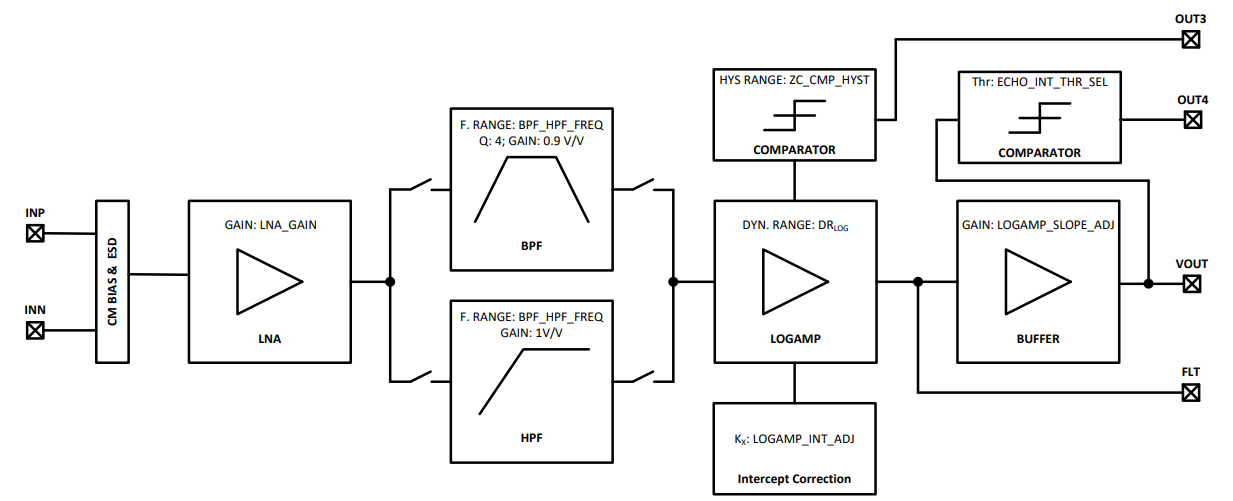
\includegraphics[width=10cm]{figure/Analog Front-End Block Diagram.png}
	\caption{回波接收模块\upcite{TUSS4470芯片手册}}
	\label{回波接收模块}
\end{figure}\par
按照TUSS4470芯片手册,我们设计了相应外围电路,如图\ref{TUSS4470芯片外围电路}所示。
\begin{figure}[!h]
	\centering
	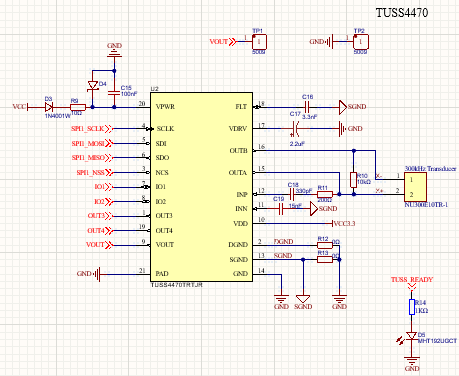
\includegraphics[width=9cm]{figure/TUSS4470 peripheral circuit.png}
	\caption{TUSS4470芯片外围电路}
	\label{TUSS4470芯片外围电路}
\end{figure}
\newpage
\subsubsection{VPWR引脚电路}
VPWR引脚输入电压范围为5V到36V,TUSS4470设备可能受到电池瞬变和反向电流的影响,因此采用外部组件保护芯片十分必要。图\ref{VPWR引脚}中除了靠近引脚的电容C15,二极管D3、D4和电阻R9就起到了保护芯片的作用。
\begin{figure}[ht]
	\centering
	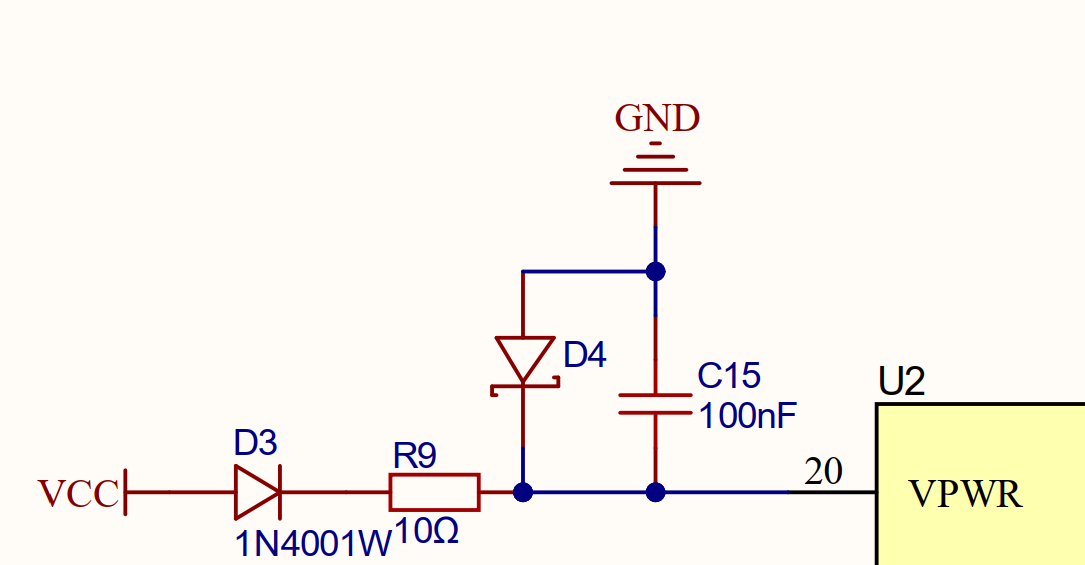
\includegraphics[width=10cm]{figure/VPWR PIN.png}
	\caption{VPWR引脚电路}
	\label{VPWR引脚}
\end{figure}
\subsubsection{FLT外接滤波电容}
FLT引脚外接滤波电容,对应图\ref{TUSS4470芯片功能框图}回波检测模块中的低通滤波器。该滤波电容的作用在于,去除对数放大器输出中的高频信号,使解调包络信号有足够的峰值保持时间,而截止频率的大小则由FLT引脚的阻抗以及外接电容的电容量所决定,该电容虽然可以抑制高频信号的波动,但同样会减缓信号的响应速度。大电容量可以使VOUT引脚输出的电压峰值变化减小,并且减缓上升下降到峰值的时间,而最优电容量则需在应用中不断进行优化。本设计初步使用电容量为3.3nF的电容。
\subsubsection{VDRV引脚电路}    
VDRV引脚连接外部电容,TUSS4470芯片通过VPWR引脚为外部的电容充电,当其达到设定电压时则停止充电,此时该电容将为超声换能器H桥驱动电路供能。
\subsubsection{超声换能器驱动电路}
在TUSS4470的芯片手册中,超声换能器有四种不同的驱动方式,不同驱动方式产生脉冲的方式也不同,本设计中采用最典型的HALF\_BRG\_MODE\_0来进行驱动,如图\ref{参考配置方式}为参考配置方式,图\ref{实际配置方式}为本设计中所采用的方式。

\begin{figure}[ht]
	\centering
	\subfloat[参考配置方式\upcite{TUSS4470芯片手册}]{
		\begin{minipage}[b]{0.5\textwidth}
			\centering
			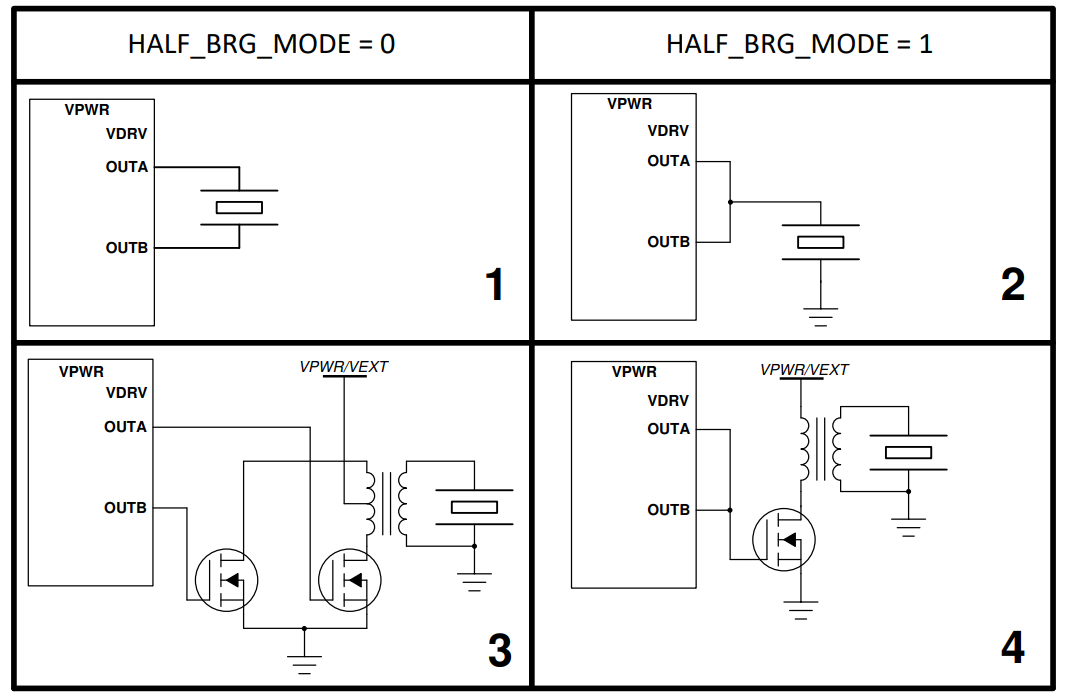
\includegraphics[height=4cm]{figure/TUSS4470 Transducer Drive Options.png}
		\end{minipage}
		\label{参考配置方式}
	}
	\subfloat[实际配置方式]{
		\begin{minipage}[b]{0.5\textwidth}
			\centering
			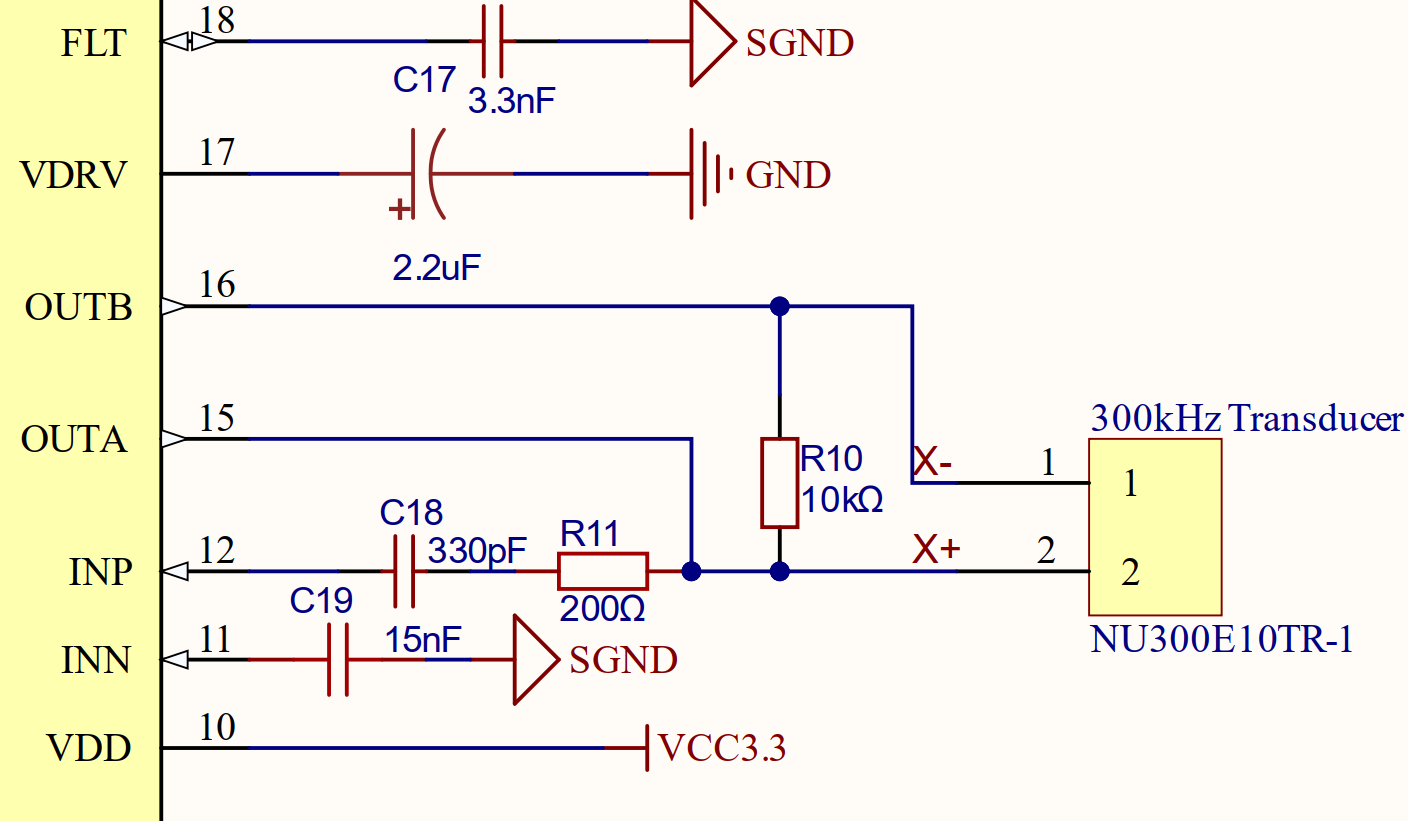
\includegraphics[height=4cm]{figure/OUTA PIN.png}
		\end{minipage}
		\label{实际配置方式}
	}
	\caption{超声换能器驱动电路设计}
	\label{超声换能器驱动电路设计}
\end{figure}
\subsubsection{芯片配置指示电路}
CPLD芯片通过SPI协议向TUSS4470芯片发送配置数据,并接收其反馈回数据。在芯片返回的数据当中,有一位的状态位用来反映芯片是否准备就绪,当芯片准备就绪后该位置1,MCU通过检测该位状态判断芯片是否准备就绪,当芯片就绪时,指示灯亮。
\subsubsection{分离接地电路}
由于外围电路中包含多种类型的信号,例如VPWR引脚的电源信号、VOUT引脚的模拟信号和SCLK等引脚的数字信号。当产生SCLK引脚产生脉冲时,其变换速度较快,会产生较大的噪声。而模拟信号又容易受到外界干扰,如果将数字信号和模拟信号直接接入同一个大地,将会严重影响模拟信号的准确性,对于超声波传感器而言,是非常致命的。本设计在原理图设计的过程中便解决了不同类型分离接地\upcite{分离接地}的问题,采用的方法是:先将不同类型的信号连接到0$\Omega$电阻,再连接到大地。使用0$\Omega$电阻可以约束电流在电路中的流动,从而起到抑制噪声的作用。起分离接地作用的电路如\ref{分离接地电路}所示。
\begin{figure}[!h]
	\centering
	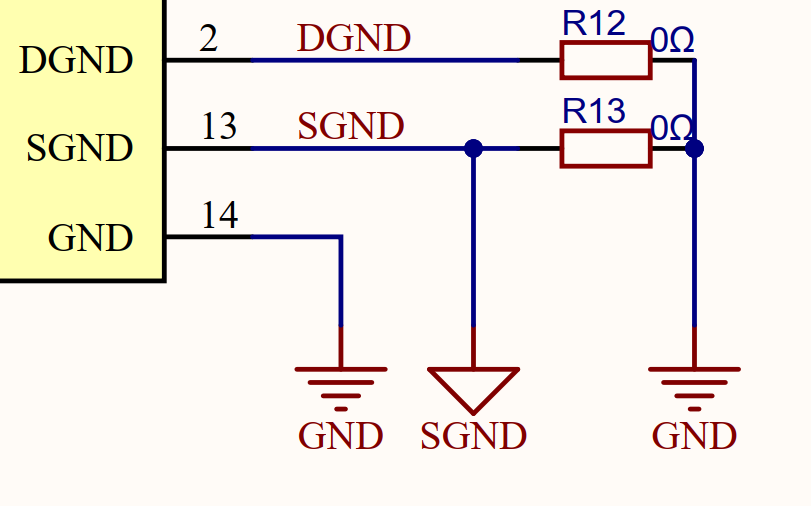
\includegraphics[width=7cm]{figure/seperate ground.png}
	\caption{分离接地电路}
	\label{分离接地电路}
\end{figure}
\subsubsection{TUSS4479芯片外围电路PCB设计}
由于本设计中涉及到的信号类型较多,包括了数字信号、模拟信号、高频信号、大功率信号,各信号间会存在较大的干扰,因此在布线过程中将各信号分离十分重要,直接关系到传感器的稳定性和精度。图\ref{TUSS4470芯片外围电路PCB设计}是TUSS4470芯片外围电路的PCB设计,图\ref{TUSS4470芯片引脚图}为芯片对应的引脚图。本设计采用两层板来完成布线。
\begin{figure}[!h]
	\begin{minipage}[t]{0.5\linewidth}
		\centering
		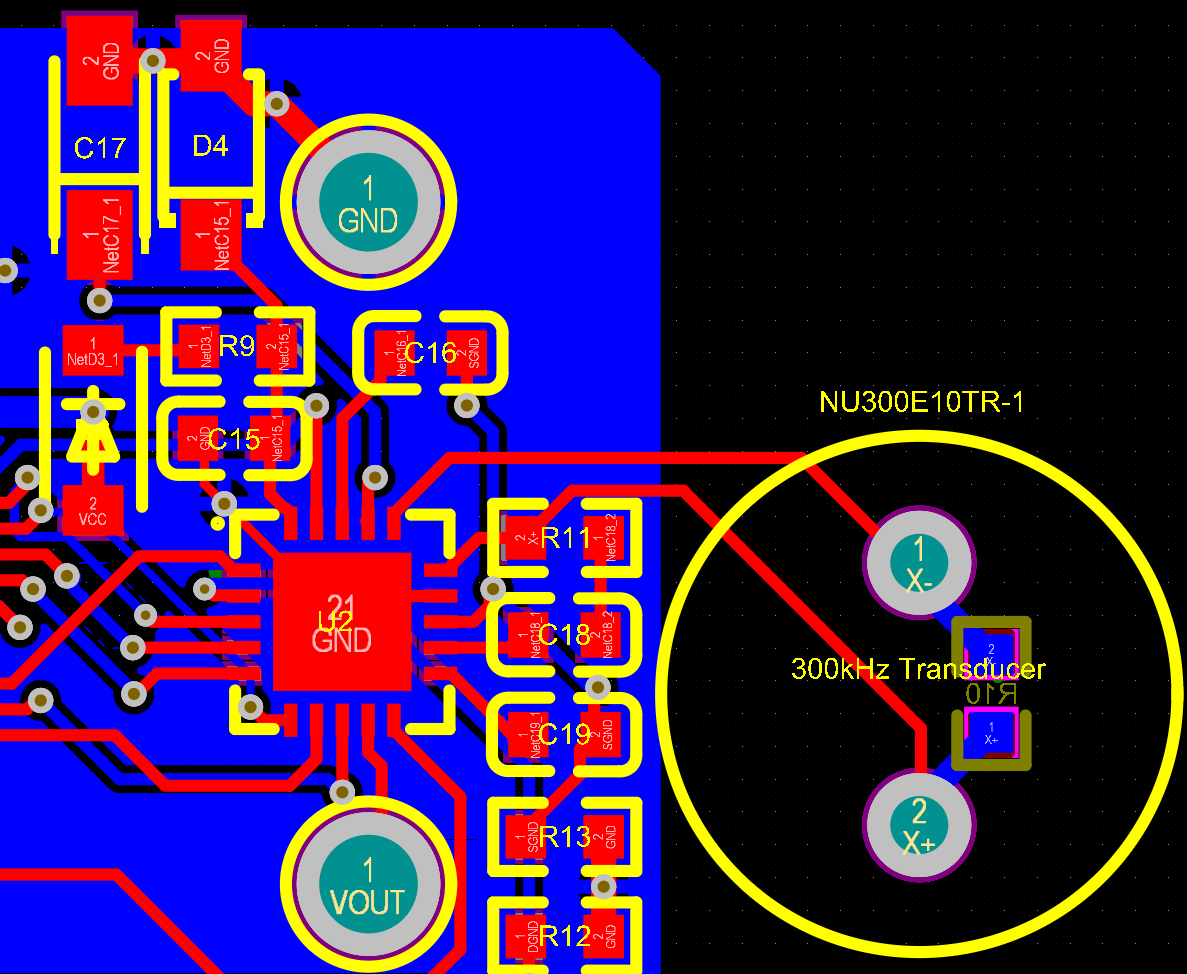
\includegraphics[height=5cm]{figure/TUSS4470 pcb.png}
		\caption{TUSS4470芯片外围电路PCB设计}
		\label{TUSS4470芯片外围电路PCB设计}
	\end{minipage}
	\begin{minipage}[t]{0.5\linewidth}
		\centering
		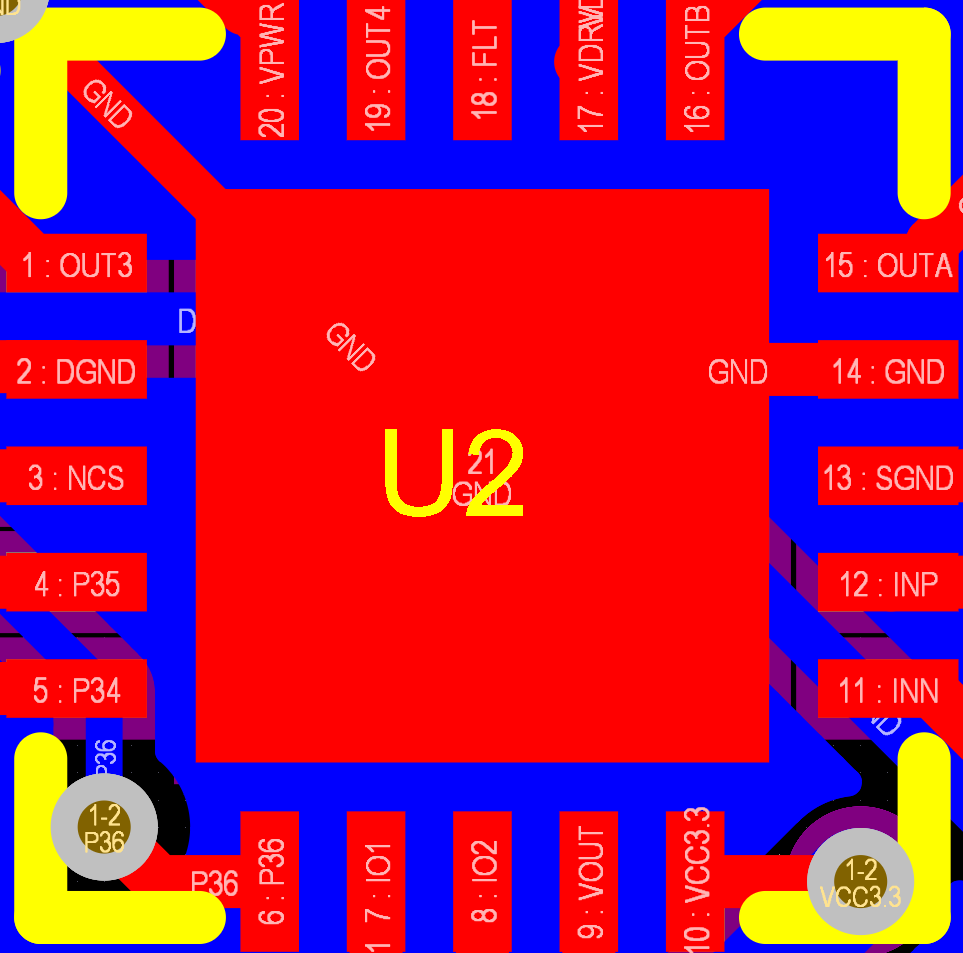
\includegraphics[height=5cm]{figure/TUSS4470 PIN.png}
		\caption{TUSS4470芯片引脚图}
		\label{TUSS4470芯片引脚图}
	\end{minipage}  		 
\end{figure}\par
在TUSS4470驱动芯片的PCB设计过程中,参考芯片手册\upcite{TUSS4470芯片手册},布线时考虑到了如下事项。\par
\paragraph{各类信号分离接地}
在连接到主地前,数字接地、传感器接地、回波接地都要先通过0$\Omega$电阻或者铜迹线,如图\ref{分离接地电路},本设计在原理图设计时采用了0$\Omega$电阻的方式来实现分离接地,因此在布线时就不需要考虑该问题。
\paragraph{回波接收引脚}
INN、INP引脚作为回波信号的接收引脚,对噪声干扰十分敏感,所以其布线必须要短且直,并且保证INN引脚的电容尽量靠近芯片引脚,以减少干扰,但考虑到后续需手工焊接,电容与芯片引脚间仍要保持一定的间隙,以减小手工焊接的难度。假设不考虑测试成本,采用贴片工艺,电容与芯片引脚间的距离还可再进一步减小,以获得到具有更高稳定性的回波信号。
\paragraph{VOUT引脚}
VOUT引脚作为模拟信号输出端,与外界的连线应该尽量短直,避免产生寄生效应\upcite{寄生效应},以及外部噪声干扰引起的噪声耦合。\par
\paragraph{超声换能器驱动}
芯片与OUTA、OUTB引脚间的布线应尽可能短且直,以保证发出脉冲信号的质量,从而提高传感器的精度。考虑到两个引脚输出的是大功率、高频率的模拟信号,连接到两引脚的线宽应不能太小。\par
\paragraph{VPWR引脚}
根据芯片手册推荐,VPWR的解调电容应尽可能靠近引脚。\par
\paragraph{信号分离}
数字信号引脚如TXD、RXD、 SCLK、 NCS、IO1、 IO2、 OUT3、OUT4应远离模拟信号引脚,避免信号间的干扰。\par
\subsection{本章小结}
本章主要介绍了超声波接近传感器硬件部分的设计,首先介绍了超声波接近传感器控制电路的设计,重点讲解了JTAG下载模块的设计和时钟包地处理。然后又详细介绍了TUSS4470芯片外围电路的设计,该部分讲解了各管脚连接器件的选型以及PCB设计过程中需要注意的事项,原理图设计部分详细介绍了VPWR引脚、VDRV引脚以及各类信号分离接地处理的设计,而PCB设计部分则详细介绍了各类器件的布局原则,以减少信号间的相互干扰。\par
至此已介绍完成了超声波接近传感器硬件设计部分的工作,下一章将详细讲解传感器的软件设计部分。




